\documentclass[sigconf, nonacm]{acmart}
\usepackage{pvldb}
\usepackage{amsmath,mathtools}
\usepackage{booktabs,graphicx,xcolor}
% Permit ordinary paragraph reflow without altering the official type size or margins.
\setlength{\emergencystretch}{2em}
\renewcommand\vldbdoi{XX.XX/XXX.XX}
\renewcommand\vldbpages{XXX-XXX}
\renewcommand\vldbavailabilityurl{https://github.com/xingxiaoyang-888/ACL-HCT}
\definecolor{draftamber}{HTML}{9A5415}
\newcommand{\draftnote}[1]{\par\smallskip\noindent{\color{draftamber}\textbf{Draft status.} #1}\par\smallskip}
\newcommand{\R}{\mathbb R}
\newcommand{\E}{\mathbb E}
\newcommand{\norm}[1]{\lVert #1\rVert}
\newcommand{\ip}[2]{\langle #1,#2\rangle_L}
\newcommand{\Acc}{\operatorname{Acc}}
\newcommand{\Var}{\operatorname{Var}}
\newcommand{\Cov}{\operatorname{Cov}}
\newcommand{\softmax}{\operatorname{softmax}}
\newtheorem{observation}{Observation}
\newtheorem{proposition}{Proposition}
\begin{document}
\title{From Neighbor Samples to Predictions: An Operator-Aware Study of GNN Quality and Inference Cost [Experiment, Analysis \& Benchmark]}
\author{Author information to be supplied}
\affiliation{\institution{Affiliation to be supplied}\country{Country to be supplied}}
\renewcommand{\shortauthors}{Author information to be supplied}
\begin{abstract}
Neighbor sampling approximates graph neural network inference, but better local estimation need not improve predictions or reduce complete request cost. We study this mismatch using paired interventions that restore local computation, upstream representations, or both, and connect their effects to finite prediction margins and native operators. Our comparison covers Uniform and LABOR on HGCN, HyboNet, GraphSAGE and GAT over ogbn-arxiv, plus GraphSAGE on PubMed, with three seeds and label-free budget selection. Restoration depends on both model and sampler: on PubMed, Uniform local restoration changes accuracy by $-0.042$ percentage points, whereas joint restoration adds $0.492$ points, exposing a positive interaction that single-layer attribution misses. LABOR also produces lower local error but $0.325$ points lower diagnostic accuracy for one PubMed seed. For identical 48,603-node arxiv workloads, exact GraphSAGE computation is approximately $235\times$ faster than middle-tier Uniform sampling (0.184 versus 43.202 seconds), using 891 MiB of peak GPU memory. Paid output reuse further reduces repeated-workload cost. These findings yield an operator-aware account of prediction loss and a quality--time--memory decision guide for choosing between sampled inference, exact computation and output reuse.
\end{abstract}
\maketitle
\vldbtopmatter

\section{Introduction}
Graph inference turns relational data into scores used by downstream applications. Recommender platforms refresh embeddings and rank candidates; enterprise graph pipelines repeatedly score a specified population under a fixed model. PinSage and AliGraph demonstrate the practical importance of graph-based recommendation and large-scale graph processing \cite{ying2018pinsage,zhu2019aligraph}. For a scoring pipeline, the systems objective is concrete: deliver the requested predictions at sufficient quality, within a memory ceiling and a completion-time budget. The execution route determines both the computational bill and which predictions are delivered.

Neighbor sampling is central to scalable GNN training, but a training execution plan is not automatically the best inference plan. During training, sampling limits dependency expansion while weights change. During a fixed-model scoring job, dependencies can be shared across targets and exact outputs can be reused until the inputs or model change. Data preparation and movement are first-class costs in GNN systems \cite{yuan2024comprehensive,kaler2022salient}. Reducing sampled edges can still leave hundreds of separate preparations, while a feasible exact pass shares work across the entire target set. At the same time, a statistically better local estimator can change the wrong predictions. Choosing a route therefore requires connecting approximation mechanisms to task decisions and complete-workload cost.

We ask: \emph{why do neighborhood samplers change prediction quality and actual cost differently across GNNs?} Four questions organize the study: Is prediction loss introduced locally or inherited from earlier layers? Why can a smaller local estimation error fail to improve decisions? Which mechanisms recur across operators, and which require a particular head? Which route best serves the same outputs under quality, memory and reuse constraints?

We study Uniform and LABOR on HGCN, HyboNet, GraphSAGE and GAT over ogbn-arxiv, plus GraphSAGE on PubMed. A historical comparison of 24 checkpoints additionally exposes training-regime sensitivity. Three findings shape the inference decision: local/upstream ordering changes with the model and sampler; restoring a local computation can hurt while restoring it jointly with the prefix helps; and lower local error can accompany more classification mistakes. Execution cost is equally consequential. For the same 48,603 arxiv outputs, exact GraphSAGE inference takes 0.184 seconds versus 43.202 seconds for middle-tier Uniform sampling---approximately $235\times$ faster, with an 891 MiB peak working set. Repeated requests create a further opportunity for paid output reuse.

We make three contributions. \textbf{A paired diagnostic of prediction loss} separates current-layer computation, upstream representations and their interaction, using signed margins and corrected/harmed decisions to explain accuracy changes. \textbf{An operator-aware analysis} connects finite error propagation to decision-sensitive directions and the native aggregation/head contract; cross-model and second-graph experiments test its implications. \textbf{A workload-level decision guide} connects prediction quality to measured request time, memory and the crossover to paid output reuse. Together, these contributions explain how an approximation changes both the predictions and the execution cost of fixed-model batch scoring.

\section{Prediction Workload and Decision Scope}
\label{sec:workload}
\paragraph{Two workload semantics lead to different execution choices.}
\emph{Capacity-constrained training} processes a large graph through repeated optimization steps: weights change and neighborhood expansion can exceed device capacity. Sampling is an important solution, alongside partitioned and out-of-core execution \cite{wan2022bnsgcn,waleffe2023mariusgnn,wang2023mgg}. Its objective includes optimization progress and data access across training iterations.

\emph{Versioned batch node scoring} instead serves an ordered target set $T$ for fixed graph topology, features and weights. Examples include scheduled embedding/output refresh, a recommendation candidate population, or a risk-scoring batch over a business graph snapshot. The relevant unit is the complete target set, including all of its batches. This paper measures that unit through static node classification. A departmental or extracted graph may fit a single 16--80~GB device. Establish residency from its edges, features, hidden states, operator and measured peak memory; this physical qualification defines the feasible inference routes.

\paragraph{Three routes implement the same scoring contract.}
Sampled inference constructs dependency cones per target batch and approximates the predictor. Exact inference computes full-neighborhood outputs and returns the requested rows. Exact-output reuse pays an initial full computation and host-cache construction, then gathers rows while the graph, features and weights retain the same version. This cache is a materialized prediction result. Streaming updates and new-node serving use different validity/recomputation contracts, as illustrated by D3-GNN and OMEGA \cite{guliyev2024d3gnn,kim2026omega}.

\paragraph{Execution-policy consequence.}
\textbf{Choose the inference route for the scoring workload, rather than inheriting the training plan by default.} When an exact pass fits and many outputs are requested, its shared computation must compete with the sum of sampled preparations, transfers and forwards. When unchanged requests repeat, paid output reuse must also compete. The choice is constrained by task quality, working memory, completion time and the valid reuse horizon. A comparison of one sampled batch with an entire exact pass would answer a different question. Our measurements support complete-target batch jobs; interactive arrival latency and update processing have their own workload contracts.

\section{Related Work}
\label{sec:scope}
\paragraph{Native operators and statistical sampling.}
GraphSAGE learns sampled neighborhood aggregators \cite{hamilton2017inductive}, GAT learns feature-dependent attention \cite{velickovic2018graph}, and HGCN and fully hyperbolic networks introduce different geometric operators \cite{chami2019hyperbolic,chen2022fully}. FastGCN, LADIES and LABOR address estimator or training efficiency through importance, layer-dependent or coordinated sampling \cite{chen2018fastgcn,zou2019ladies,balin2023labor}. Our question follows the resulting approximation through a frozen native operator to its predictions. Depth, normalization and heads remain part of that contract; cross-architecture differences alone cannot identify curvature.

\paragraph{Data access and sampled execution.}
DGL and PyG provide graph execution and mini-batch abstractions \cite{wang2019dgl,fey2019pyg}. GraphBolt makes sampling, feature fetching and device copying explicit pipeline stages \cite{dgl2024graphbolt}. Their end-to-end cost matters beyond a forward kernel. GNNLab factors sampling and training across GPUs \cite{yang2022gnnlab}; SALIENT optimizes sampling, preparation and transfer \cite{kaler2022salient}; BGL targets graph I/O and preprocessing \cite{liu2023bgl}. PaGraph uses computation-aware feature caching \cite{lin2020pagraph}; DUCATI divides GPU cache capacity between adjacency and features \cite{zhang2023ducati}; Legion coordinates multi-GPU caching and partitioning at billion-graph scale \cite{sun2023legion}. NeutronOrch revisits CPU--GPU task placement and bounded historical-embedding reuse \cite{ai2024neutronorch}. The comprehensive PVLDB evaluation identifies data management as a major determinant of GNN training performance \cite{yuan2024comprehensive}. These works establish why preparation, communication and reuse belong in the cost model. Our contribution adds fixed-model prediction consequences and a same-output inference comparison; it is complementary to optimizing these engines.

\paragraph{Full-graph execution and capacity.}
GNNAdvisor adapts GPU work mapping and memory management to GNN workloads \cite{wang2021gnnadvisor}. MGG pipelines fine-grained communication and computation across GPUs \cite{wang2023mgg}; BNS-GCN reduces communication in partition-parallel training using boundary-node sampling \cite{wan2022bnsgcn}. MariusGNN addresses out-of-core training and sampled dependency redundancy \cite{waleffe2023mariusgnn}. Thus capacity pressure admits multiple execution strategies, each with a particular computation and quality contract. Our resident exact baseline tests one feasible route, rather than treating full-neighborhood computation as necessarily unavailable.

\paragraph{Inference, serving and reuse.}
PinSage and AliGraph connect graph computation to production recommendation and graph platforms \cite{ying2018pinsage,zhu2019aligraph}. Channel pruning studies full and batched GNN inference with hidden-feature caching \cite{zhou2021channel}; DGI reorganizes inference layer by layer \cite{yin2022dgi}. OMEGA combines selective recomputation with distributed serving \cite{kim2026omega}, while D3-GNN maintains streaming graph computations through dynamic dataflow \cite{guliyev2024d3gnn}. These systems motivate explicit target coverage and validity periods. Our exact-output cache stores the final predictions of one unchanged version. Historical hidden-state reuse during optimization has a different contract, as in variance-reduced training, GNNAutoScale and Pseudo Full Neighborhood Compensation \cite{chen2018stochastic,fey2021gnnautoscale,zhou2025faster}.

\paragraph{Evidence and contribution boundary.}
Jendal et al. evaluate graph samplers for inductive recommender training \cite{jendal2025limits}; our paired interventions examine frozen node-classification predictors. We combine a message-passing analysis framework, conditional native-operator derivations and named empirical observations. The distinctive connection is from local/upstream restoration to signed decision changes and then to the quality--time--memory choice for a complete scoring job. Estimator quality, diagnostic recoverability and deployment value are measured separately, with training-regime comparisons retained as a distinct evidence stream.

\section{From Local Sampling to Task Decisions}
\label{sec:analysis}
Using the standard message-passing abstraction \cite{gilmer2017neural}, our diagnostic asks which part of a fixed prediction computation must change to remove an observed loss. We first hold the checkpoint and target nodes fixed, then separate local computation from incoming representations, interpret the resulting decision changes under the native head, and compare deployable routes on the same requested outputs. Three analytical insights organize the connection to the experiments. The supplement supplies full expansions, estimator conditions and exact implementation anchors.

\subsection{Controlled local and upstream interventions}
At the final message layer, let $X$ contain messages from the exact prefix and $\widehat X$ messages from the sampled prefix. Let $f_0$ be the native sampled layer and $f_1$ the native full-neighborhood layer, including its weighting, normalization and activation. The four states are
\begin{align}
H_{00}&=f_0(\widehat X), & H_{10}&=f_1(\widehat X),\\
H_{01}&=f_0(X), & H_{11}&=f_1(X).
\label{eq:corners}
\end{align}
The first index restores local computation; the second restores the upstream representation. Each branch uses the same checkpoint, targets and native head, and sampled branches share the prescribed plan. In GAT, local restoration recomputes full-neighborhood attention on the \emph{same incoming states}; it does not borrow weights computed from a different prefix.

For quality $Q$, local, upstream and joint changes are $Q_{10}-Q_{00}$, $Q_{01}-Q_{00}$ and $Q_{11}-Q_{00}$. Their interaction is
\begin{equation}
I_Q=Q_{11}-Q_{10}-Q_{01}+Q_{00}.
\label{eq:interaction}
\end{equation}
Thus joint change equals local change plus upstream change plus $I_Q$. This is the standard two-factor interaction contrast \cite{nist2012handbook}. Accuracy thresholds can make it nonzero even for linearly combined representations; exact computation defines the reference predictor, while labels determine correctness.

\paragraph{\normalfont\bfseries Analytical Insight 1 (Context-dependent recovery).}
The local gain is $Q_{10}-Q_{00}$ on a sampled prefix and $Q_{11}-Q_{01}$ on an exact prefix; their difference is precisely $I_Q$. On PubMed/Uniform these gains are $-0.0417$ and $+0.2167$ percentage points: changing the upstream context turns local restoration from harmful to helpful, with $I_Q=+0.2583$ points. This complementarity makes the four-branch diagnostic essential: attributing the joint gain to isolated local and upstream effects omits the measured interaction.

The diagnostic uses complete whole-graph prefixes, preserving the chosen incoming states at every destination. Deployment evaluation uses target dependency cones. We report these sampling distributions separately and account for the exact states and support traces as diagnostic costs.

\subsection{Interpreting propagation and prediction changes}
For an exact layer $F_\ell$, sampled layer $\widehat F_\ell$ and representation change $\delta_\ell=\widehat H_\ell-H_\ell$, define
\begin{align}
e_\ell&=\widehat F_\ell(\widehat H_{\ell-1})-F_\ell(\widehat H_{\ell-1}),\\
\delta_\ell&=J_\ell\delta_{\ell-1}+e_\ell+r_\ell,
\label{eq:prop}
\end{align}
where $J_\ell$ is any selected linear map and $r_\ell=F_\ell(\widehat H_{\ell-1})-F_\ell(H_{\ell-1})-J_\ell\delta_{\ell-1}$. Keeping this residual makes the decomposition finite and exact. With identical raw inputs, repeated substitution gives
\begin{equation}
\delta_L=\sum_{\ell=1}^{L}P_{L:\ell+1}(e_\ell+r_\ell),
\qquad P_{L:\ell+1}=J_L\cdots J_{\ell+1},
\label{eq:unrolled}
\end{equation}
where the empty product is the identity. This separates newly introduced local error from the transformations applied to earlier errors. It neither assumes independent errors nor determines the signs of their decision effects. A complete final neighborhood can have $e_L=0$ while $\delta_L\ne0$. Conversely, a one-message-layer model with identical raw inputs has no sampled upstream message-passing prefix. These are precisely the distinctions tested by the four branches: restoring the last neighborhood removes its new approximation, whereas restoring the prefix changes the inputs on which that neighborhood operates.

On a differentiable branch, choosing $J_\ell=DF_\ell(H_{\ell-1})$ permits the standard Taylor interpretation \cite{nocedal2006numerical}. If the Jacobian is $K_\ell$-Lipschitz along the whole segment between the two inputs, integration of the Jacobian difference yields
\begin{equation}
\norm{r_\ell}\leq\tfrac12K_\ell\norm{\delta_{\ell-1}}^2.
\label{eq:remainder}
\end{equation}
The condition applies along a valid coordinate segment within a differentiable branch. Our interventions evaluate the finite native maps, including attention, activations and normalization; they use the exact residual form rather than estimated smoothness constants.

For scores $s_c$, the true-class margin is $m_y=s_y-\max_{c\ne y}s_c$. For a named affine head $s_c(h)=w_c^\top h+b_c$, write $M_{ab}=s_a-s_b$. Direct subtraction for a finite change $d$ gives
\begin{equation}
M_{ab}(h+d)-M_{ab}(h)=(w_a-w_b)^\top d.
\label{eq:euclideanmargin}
\end{equation}
The direction of $d$ relative to a boundary matters, not its norm alone. For a correctly classified node, a sufficient stability condition is
\begin{equation}
\max_{c\ne y}|(w_y-w_c)^\top d|<m_y(h).
\label{eq:stability}
\end{equation}
The bound exposes the relevant direction. With a binary margin of $0.1$ and class-weight difference $(1,0)$, perturbation $(-0.2,0)$ reverses the decision, whereas the larger perturbation $(0,1)$ leaves the margin unchanged. This separates decision sensitivity from squared error. The strongest competing class can also switch. We therefore report native margins and paired corrected/harmed events, whose net effect is
\begin{equation}
\Acc_{\mathrm{intervention}}-\Acc_{00}=(C-H)/N.
\label{eq:transitions}
\end{equation}
Here $N$ is the same node--plan event set in both branches. A mean margin can improve while more nodes become wrong: accuracy is determined by the individual boundary crossings counted in $C$ and $H$.
\paragraph{\normalfont\bfseries Analytical Insight 2 (Decision-sensitive error, not error size).}
Equations~\eqref{eq:unrolled}--\eqref{eq:stability} identify the relevant chain: propagated perturbation, projection onto class boundaries and the original margin. A local norm omits the latter two. PubMed/LABOR seed 37 has smaller measured local error yet loses 0.325 accuracy points and 0.03629 in mean native margin. Reporting signed margins and paired corrections/harms therefore supplies decision information that estimator error alone discards. This within-model observation concerns the complete sampled computation; each sampler retains its own incoming states.

\subsection{Preserving the operator's estimator contract}
Uniform's fixed-size nonempty sample mean is unbiased for fixed messages; this property does not imply unbiased network outputs. LABOR's layer-level coordination and estimator result \cite{balin2023labor} must likewise be matched to the actual implementation. Our LABOR-0 SAGE path divides by its random realized count and returns zero for an empty neighbor term; nonempty returned importance weights are rejected. It therefore does not inherit the fixed-count argument. The separate root transform remains present even when the neighbor term is zero.

Hyperbolic support uses a fixed self contribution and a Horvitz--Thompson-weighted non-self sum \cite{horvitz1952generalization} before the native nonlinear map. For fixed messages $x_j$, inclusion indicators $I_j$ and correct positive marginal probabilities $\pi_j$, the linear identity is
\begin{equation}
\E\!\left[\sum_j I_j a_jx_j/\pi_j\,\middle|\,X\right]=\sum_j a_jx_j.
\label{eq:ht}
\end{equation}
Joint inclusion probabilities determine its covariance. Applying it to a sampled upstream state requires its conditional sampling law to retain the stated probabilities; shared randomness cannot silently be treated as independence. Subsequent log/exp or Lorentz normalization is a different mathematical object.

GAT keeps one self message and sampled-neighborhood softmax. For full attention $a=N/D$ and sampled numerator/denominator differences $\delta N,\delta D$, direct subtraction gives
\begin{equation}
\widehat a-a=\frac{\delta N-a\,\delta D}{D+\delta D}.
\label{eq:attentionratio}
\end{equation}
Even separately unbiased numerator and denominator estimates need not give an unbiased ratio. Our native sampled softmax adds no inverse-probability attention correction. The supplement gives the standard delta-method approximation \cite{oehlert1992delta}, requiring centered perturbations, a denominator bounded away from zero and a controlled remainder. The experiments measure the resulting native outputs and decisions rather than substituting that approximation for observations.

The HyboNet head provides a more specific illustration \cite{chen2022fully}. Its native aggregate is normalized by $\rho(m)=\sqrt{\max\{|\ip{m}{m}|,10^{-8}\}}$, and its scores are $s_c=2+2\ip{m/\rho}{p_c}+b_c$. For $D_{ab}=p_a-p_b$ and $\beta_{ab}=b_a-b_b$, positive $\rho$ preserves margin sign and gives
\begin{equation}
\psi^\rho_{ab}(m)=\rho(m)M_{ab}=2\ip{m}{D_{ab}}+\rho(m)\beta_{ab}.
\label{eq:psi}
\end{equation}
\begin{align}
\psi^\rho_{ab}(m+d)-\psi^\rho_{ab}(m)
={}&2\ip{d}{D_{ab}}\notag\\
&+[\rho(m+d)-\rho(m)]\beta_{ab}.
\label{eq:lorentzfinite}
\end{align}
\paragraph{\normalfont\bfseries Analytical Insight 3 (Bias-conditioned Lorentz scale invariance).}
With equal class biases, the positive scalar normalization cancels from pairwise class order for a fixed aggregate: Equation~\eqref{eq:psi} reduces its sign to that of $\ip{m}{D_{ab}}$. A correction that only changes this common scale leaves predictions unchanged. Changing the aggregate can still alter its class-discriminating projection; with unequal biases, Equation~\eqref{eq:lorentzfinite} also retains the finite normalization change. This pinpoints when geometric normalization error can affect decisions and when it cannot. The measured HyboNet branches preserve their actual trained biases and aggregate changes, so recovery reflects their joint effect.

The factorization follows directly from the native HyboNet head \cite{chen2022fully}, for finite fixed prototypes/biases and a positive floored denominator in real arithmetic. Its ideal hyperboloid interpretation additionally requires future-timelike aggregates above the floor and unit future-pointing prototypes. The supplement relates these conditions to FP32 execution and distinguishes chordal from geodesic quantities. HGCN's affine decoder instead follows the preceding margin analysis.

\section{Comparing Complete Prediction Workloads}
\label{sec:cost}
Let $T$ be an ordered target-node workload with a fixed batching rule. Every route must serve the same requested outputs. Timed sampled inference includes neighborhood planning, block construction, host--device movement and synchronized forward computation. Graph/checkpoint loading, format construction and warm-ups are recorded separately. End-to-end timing measures the complete request directly; phase intervals describe its components. Equal fanout can entail different costs because sharing, duplicates, attention and preparation differ.

We select three discrete budgets by label-free timing, then report each route's final quality, complete-workload time and GPU-memory peak. Budgets remain fixed during final scoring. Dominance is defined over feasible measured points in the reported dimensions; the quality--cost plots display the resulting discrete operating choices.

For $q$ repetitions of the same workload, sampled computation pays $C_s(q)=S_s+qT_s(T)$, whereas a cached exact output pays
\begin{equation}
C_c(q)=S_f+P_f+qT_c(T),
\label{eq:cache}
\end{equation}
with route setup $S$, full-output construction $P_f$ and cached gather $T_c$. When $T_s(T)>T_c(T)$, elementary cost comparison makes caching cheaper for
\begin{equation}
q>\frac{S_f+P_f-S_s}{T_s(T)-T_c(T)}.
\label{eq:breakeven}
\end{equation}
The strict inequality determines the smallest admissible integer; a nonpositive denominator does not support this crossover argument. CPU cache bytes, GPU working memory and invalidation after graph or weight changes are part of the decision. A full-graph forward is not compared with a single small sampled batch: both routes serve the identical complete $T$.

The accounting separates common residency from route-specific work. A resident graph and loaded checkpoint are shared preconditions; their loading costs are recorded separately. Exact inference pays for format setup, full output construction and target gathering. RAM reuse pays for the first full computation and transfer to host memory, then for each gather. Repeated exact computation pays for each new full forward. Recorded components define the $q=1,10,100$ values and the continuous cost-model curves between them.

\section{Experimental Protocol}
\label{sec:protocol}
\subsection{Frozen models, graphs and targets}
The comparison uses plain three-layer HGCN, HyboNet, GraphSAGE and GAT checkpoints on ogbn-arxiv \cite{hu2020open}, plus three-layer GraphSAGE on PubMed \cite{yang2016revisiting}, with seeds 11, 23 and 37 in every group. The 12 arxiv base checkpoints precede the later correction adaptations and are reused unchanged. PubMed adds three fixed-configuration 500-epoch base trainings. Checkpoints, samplers, budgets, intervention locations, metrics and statistical rules were fixed before the single final official-test evaluation.

\begin{table*}[tp]
\centering\small
\caption{Frozen model and operator scope. Every new group has three message layers and seeds 11/23/37. The four arxiv groups reuse original plain checkpoints; only PubMed/SAGE requires new base training. Matching seeds and depth does not match all architecture or training choices.}
\label{tab:model-contracts}
\begin{tabular}{p{.12\textwidth}p{.39\textwidth}p{.40\textwidth}}
\toprule
Model & Local aggregation and prediction contract & Checkpoint and comparison scope\\
\midrule
GraphSAGE & Realized non-self mean plus separate root transform; hidden batch normalization/ReLU; final class scores and log-softmax. & Three original arxiv checkpoints; three PubMed checkpoints from fixed 500-epoch base training. Common log-softmax cancels in pairwise score differences.\\
GAT & Feature-dependent per-destination softmax, one self edge, native per-head aggregation, residual and bias. & Three original arxiv checkpoints. Restoration recomputes attention on the selected incoming state; it does not fix attention across different prefixes.\\
HGCN & Fixed-self weighted origin-tangent support followed by native hyperbolic maps; linear decoder. & Three original arxiv checkpoints. Distinct from the one-layer historical HGCN, whose upstream branch is a structural alias.\\
HyboNet & Fixed-self weighted ambient support, native Lorentz scalar normalization, prototype scores and class bias. & Three original arxiv checkpoints. The finite head identity uses the actual normalization floor; unit-hyperboloid interpretation has extra conditions.\\
\bottomrule
\end{tabular}
\end{table*}

Table~\ref{tab:model-contracts} identifies the computation preserved when sampling changes. The arxiv checkpoints use their original sampled-training contracts. PubMed uses the existing SAGE architecture, a fixed training fanout and configuration, and fit-only checkpoint selection. Within-checkpoint contrasts change a named computation; between-model contrasts additionally reflect differences in widths, normalization, heads and optimization histories.

The historical synthesis reuses 24 HyboNet/HGCN checkpoints crossing Airport/Disease-NC, full/matched training and three seeds. Historical HGCN has one message layer, whereas HyboNet has five on Airport and three on Disease-NC. The one-layer model's structural upstream alias is distinguished from the measured upstream effects in the new three-layer models. Historical records retain their original development or confirmation role.

The final workloads contain 48,603 arxiv test nodes and 1,000 PubMed test nodes. Fixed batches of 128 give 380 arxiv requests (379 full batches and 91 final nodes) and eight PubMed requests (seven full batches and 104 final nodes). Four prescribed repeats serve the same targets and ordering. Calibration uses separate frozen development targets; its request medians are not final-workload times.

PubMed provides qualified data and a contrasting graph/label structure, with 19,717 nodes and 60 training labels. The inherited native loader uses 1,000 validation nodes, split into 500 fit and 500 development nodes. Fit selects the checkpoint; development supplies label-free timing targets. Earlier hyperbolic work had evaluated PubMed test, while the present ordinary-model configuration was fixed independently of those scores. Full configurations, selected epochs and fit scores are provided in the supplement.

\subsection{Samplers, budgets and metrics}
Uniform uses per-layer fanout 5, 15 and 30 on arxiv, and 1, 4 and 8 on PubMed. LABOR-0 uses no external probability input and zero importance-sampling iterations. For each group, seed-11 label-free calibration selects the largest registered LABOR fanout whose median request time does not exceed the corresponding Uniform target; other seeds inherit it. Candidate sets and full millisecond measurements for all five budget locks, comprising 15 calibrated tier rows, are retained in the supplement and public artifact. If no point fits, the minimum is reported as infeasible, without interpolation or retiming.

SAGE/arxiv's low LABOR point exceeds its target by approximately 0.298\% and remains infeasible. PubMed selects the same LABOR $K=6$ at all three tiers; these are not three independent operating points. Its Uniform $K=8$ calibration is faster than $K=4$, and that nonmonotonicity is retained. Actual final costs can differ from the calibration match. Near-equal quality requires no seed more than 0.2 percentage points below its comparison point.

Primary quality is label accuracy. Middle-budget final-layer diagnostics record four-corner accuracy, native signed margin, corrections, harms and local-estimator error; deployment records cover every low, middle and high endpoint. Branches are paired by checkpoint, target and sampling plan. Each seed is summarized over four repeats; means and sample standard deviations are then computed across three training seeds. Error dimensions and score scales are compared within each model/dataset group.

\subsection{Experimental environment}
The main inference comparisons were run on up to four NVIDIA A800-SXM4 GPUs (80\,GB each), with one run per GPU. We report end-to-end inference time and peak allocated GPU memory for identical target workloads.

% Systems revision: original scientific scalars, revised presentation, new decision guide.
% Source-only figure slots. No fabricated axes or placeholder data are drawn.
% Root/Ops supplies accepted scalar paths/hashes to the separate render manifest.
% This output directory is a proposed manuscript destination, not a guessed input.
\providecommand{\finalfiguredir}{figures/manuscript-refresh-v3}
\newcommand{\FinalMechanismFigure}{%
\IfFileExists{\finalfiguredir/final_mechanism_restoration.pdf}{%
\begin{figure*}[tp]
\centering
\includegraphics[width=.95\textwidth]{\finalfiguredir/final_mechanism_restoration.pdf}
\caption{Final-layer restoration at the middle budget. Markers retain all three seed means over four paired repeats; the dashed line is the sampled baseline. Each U/L annotation reports the largest local/upstream/joint three-seed mean gain and the interaction $I_Q$. Panel scales can differ. Whole-graph diagnostic prefixes differ from deployment dependency cones.}
\Description{Five model and dataset panels compare accuracy changes under local, upstream and joint restoration for Uniform and LABOR. Seed markers, zero baselines and interaction annotations expose differences across configurations.}
\label{fig:final-mechanism}
\end{figure*}
}{\draftnote{Final four-corner figure awaits accepted scalar exports and controlled rendering.}}

}

\newcommand{\FinalErrorDecisionFigure}{%
\IfFileExists{\finalfiguredir/final_local_error_decision.pdf}{%
\begin{figure*}[tp]
\centering
\includegraphics[width=.95\textwidth]{\finalfiguredir/final_local_error_decision.pdf}
\caption{Within-model LABOR-minus-Uniform local-error and accuracy differences at the middle budget. Points are seed means; bars show the range of four paired-repeat differences. Native error scales compare only within a model/dataset panel. Each sampler uses its own incoming states, so the comparison describes the sampled computation rather than isolating variance at fixed inputs.}
\Description{Five scatter panels compare LABOR minus Uniform changes in local approximation error and accuracy. Each seed is a point with the range across paired repeats. Smaller estimator error does not impose a uniform accuracy ordering.}
\label{fig:final-error-decision}
\end{figure*}
}{\draftnote{The model-internal error--decision comparison awaits accepted mechanism scalar exports; no cross-model error ranking is inferred.}}

}

\newcommand{\FinalQualityCostFigure}{%
\IfFileExists{\finalfiguredir/final_quality_workload_memory.pdf}{%
\begin{figure*}[tp]
\centering
\includegraphics[width=.97\textwidth,height=.82\textheight,keepaspectratio]{\finalfiguredir/final_quality_workload_memory.pdf}
\caption{Quality, complete-target-workload time and allocated GPU memory for every seed and tier. Light L--M--H links connect the measured tiers for each seed; ! marks the infeasible calibration match. Red stars show exact computation, with seed labels. At the middle tier, exact computation is faster and uses more peak memory. Sampled time includes preparation, transfers and forward; exact pays format setup, full computation and gathering. Common loading is separate.}
\Description{Accuracy versus time and GPU memory across three sampling budgets for each model and dataset. Linked seed points show Uniform and LABOR routes; red stars mark exact computation.}
\label{fig:final-quality-cost}
\end{figure*}
}{\draftnote{Final quality--time--memory points await accepted complete-workload scalar exports. Calibration medians do not fill these axes.}}

}

\newcommand{\FinalCacheFigure}{%
\IfFileExists{\finalfiguredir/final_full_RAM_amortization.pdf}{%
\begin{figure*}[tp]
\centering
\includegraphics[width=.95\textwidth]{\finalfiguredir/final_full_RAM_amortization.pdf}
\caption{Cumulative cost models $a+bq$ for $1\leq q\leq100$. Thin lines show individual seeds; thick lines average their formulas. Uniform/LABOR use middle-tier mean workload time; exact/RAM use median-based cost components. Crosses mark intersections of the mean RAM/alternative formulas. HyboNet's RAM/full intersection is $q^*=0.974<1$, so RAM is already cheaper at $q=1$ and no crossing appears in the plotted interval. RAM pays its build; common loading is separate. Graph, features, weights and targets remain fixed.}
\Description{Cumulative time curves compare sampled inference, exact recomputation and paid RAM output reuse for repeated fixed workloads. Marked crossings identify the analytic break-even points.}
\label{fig:final-cache}
\end{figure*}
}{\draftnote{Paid full/RAM curves await accepted final scalar records at the registered $q$ values.}}
}


\newcommand{\FinalDecisionGuideFigure}{%
\begin{figure}[tp]
\centering
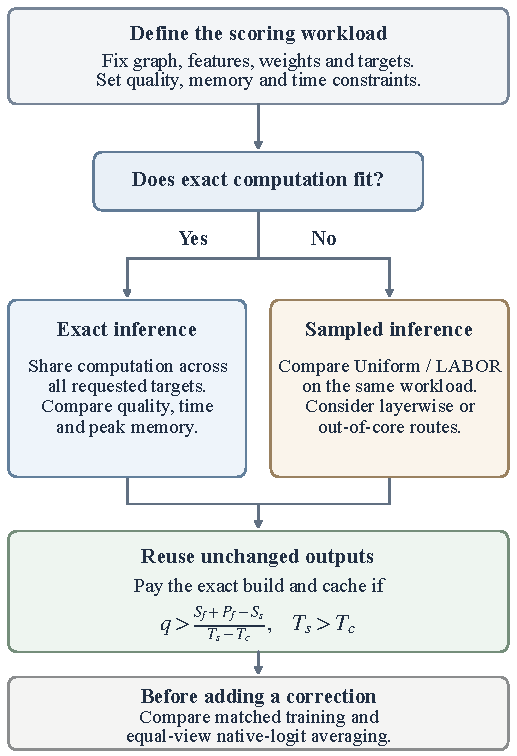
\includegraphics[width=\columnwidth]{figures/decision-guide-roman-v2/final_decision_guide.pdf}
\caption{A guide for comparing feasible prediction routes under a fixed workload and quality/memory/time constraints. Exact-output reuse requires a feasible paid build and valid cached outputs. Layerwise/out-of-core execution is a literature alternative, not evaluated here. Historical comparisons motivate matched-training and equal-view native-logit controls before a more complex correction.}
\Description{A flowchart starts from workload and quality constraints, checks output-cache validity and exact-computation feasibility, and compares feasible exact or sampled routes under measured time and memory costs.}
\label{fig:decision-guide}
\end{figure}
}


\section{Experimental Results}
\label{sec:results}
The results cover 15 model--seed cells: HGCN, HyboNet, GraphSAGE and GAT on arxiv, plus GraphSAGE on PubMed, each at seeds 11/23/37. Every cell includes both samplers at three budget tiers, middle-budget four-corner measurements, and exact/RAM costs. Complete per-seed tables accompany the model-level findings below.

\subsection{Local restoration, upstream restoration and interaction}
Figure~\ref{fig:final-mechanism} reveals model- and sampler-dependent recovery. On arxiv, Uniform local restoration exceeds upstream restoration for HGCN, HyboNet and SAGE, whereas GAT has the opposite mean ordering. LABOR reverses that ordering for HGCN and HyboNet, but not SAGE. All eight arxiv model/sampler mean joint gains are below 0.7 percentage points, locating the remaining approximation loss of these sampled-trained models. The three-layer HGCN exhibits an upstream effect that its historical one-layer counterpart cannot express.

\FinalMechanismFigure

\paragraph{Second-graph evidence changes the balance.}
On PubMed/SAGE, Uniform local restoration changes accuracy by $-0.0417$ points, upstream restoration by $+0.2750$, and joint restoration by $+0.4917$. The $+0.2583$-point interaction contrasts with the small negative mean interactions on arxiv. Local restoration corrects 2.917 and introduces 3.333 mistakes per repeat on average; joint restoration corrects 18.500 and introduces 13.583. The counts connect the interaction to actual decision changes. Seed-level exceptions further sharpen the result: PubMed/LABOR seed 23 loses 0.200 points under upstream restoration and 0.025 under joint restoration, while Uniform local restoration harms seeds 11 and 37.

Both-restored HGCN outputs retain a small LABOR-minus-Uniform mean accuracy difference of $-0.0024$ points across their floating-point execution paths. This numerical discrepancy is included in the per-seed results.

\subsection{Local estimator error and task decisions}
\FinalErrorDecisionFigure
Figure~\ref{fig:final-error-decision} compares local squared error and diagnostic accuracy within each model. The arxiv mean differences favor Uniform on both quantities, but that aggregate pattern is not a universal implication. On PubMed, LABOR reduces the measured local error for each seed; seed 37 nevertheless loses 0.325 accuracy points and its mean native margin decreases by 0.03629. Seeds 11 and 23 gain 0.250 and 0.200 points, respectively. Thus the same direction of error change has different task consequences even within a single model/dataset group.

The interventions expose the same decision sensitivity. Exact local computation on PubMed/Uniform lowers mean accuracy, but adding it after upstream restoration increases accuracy by 0.2167 points. The latter gain occurs even though the mean native margin changes by $-0.004993$. Insight 2 explains the apparent contradiction: the aggregate magnitude or mean margin hides which individual nodes cross a boundary. The paired corrections and harms recover that missing decision information.

\subsection{Quality, complete-workload time and memory}
Table~\ref{tab:final-deployment} reports the middle tier; Figure~\ref{fig:final-quality-cost} retains every low, middle and high endpoint and seed. LABOR is faster at the middle arxiv tier, but its mean accuracy is slightly lower for all four models. These are comparisons at preselected discrete operating points, not an exact equal-time competition. HGCN's U15 and L12 final workloads take 48.676 and 34.903 seconds, with 70.146\% and 69.846\% accuracy, respectively. Its seeds 11 and 23 violate the fixed 0.2-point near-equal-accuracy tolerance. HyboNet, SAGE and GAT satisfy that tolerance at their middle points, but this does not establish the same trade-off at every tier. At low budget LABOR helps HGCN (68.818 versus 67.255\%) yet hurts HyboNet (65.501 versus 67.357\%); SAGE's low LABOR point remains calibration-infeasible. At high budget the observed accuracy differences are much smaller.

\begin{table*}[t]
\caption{Final deployment at the frozen middle tier and exact $q=1$ computation on the identical complete target workload. Accuracy and time are three-seed mean $\pm$ sample standard deviation. Sampled memory is the mean of each seed's four observed peaks; exact memory includes format setup and forward. Graph/CP loading is separately reported. Discrete calibration locks do not imply equal final times. All low/high endpoints, per-seed maxima and setup fields remain in the supplement.}
\label{tab:final-deployment}
\centering
\small
\begin{tabular}{llrrrr}
\toprule
Group & Method & Fanout & Accuracy (\%) & Workload time (s) & Mean peak (MiB) \\
\midrule
HGCN / arxiv & Uniform & 15 & 70.146 $\pm$ 0.232 & 48.676 $\pm$ 0.396 & 303.1 \\
HGCN / arxiv & LABOR & 12 & 69.846 $\pm$ 0.385 & 34.903 $\pm$ 0.464 & 196.0 \\
HGCN / arxiv & Exact & all & 70.470 $\pm$ 0.300 & 0.239 $\pm$ 0.023 & 891.4 \\
HyboNet / arxiv & Uniform & 15 & 69.991 $\pm$ 0.190 & 42.362 $\pm$ 0.155 & 159.7 \\
HyboNet / arxiv & LABOR & 15 & 69.887 $\pm$ 0.181 & 35.893 $\pm$ 0.100 & 131.1 \\
HyboNet / arxiv & Exact & all & 70.165 $\pm$ 0.131 & 0.339 $\pm$ 0.055 & 482.6 \\
GraphSAGE / arxiv & Uniform & 15 & 70.858 $\pm$ 0.439 & 43.202 $\pm$ 0.204 & 107.8 \\
GraphSAGE / arxiv & LABOR & 15 & 70.826 $\pm$ 0.390 & 36.480 $\pm$ 0.194 & 90.7 \\
GraphSAGE / arxiv & Exact & all & 70.970 $\pm$ 0.398 & 0.184 $\pm$ 0.006 & 891.0 \\
GAT / arxiv & Uniform & 15 & 72.159 $\pm$ 0.089 & 44.818 $\pm$ 0.206 & 1245.8 \\
GAT / arxiv & LABOR & 15 & 72.099 $\pm$ 0.081 & 37.990 $\pm$ 0.296 & 929.5 \\
GAT / arxiv & Exact & all & 72.295 $\pm$ 0.086 & 0.299 $\pm$ 0.007 & 1977.8 \\
GraphSAGE / PubMed & Uniform & 4 & 74.858 $\pm$ 0.636 & 0.329 $\pm$ 0.002 & 48.1 \\
GraphSAGE / PubMed & LABOR & 6 & 74.975 $\pm$ 0.687 & 0.346 $\pm$ 0.014 & 53.9 \\
GraphSAGE / PubMed & Exact & all & 75.267 $\pm$ 0.611 & 0.080 $\pm$ 0.005 & 169.9 \\
\bottomrule
\end{tabular}
\end{table*}

\FinalQualityCostFigure

PubMed's middle LABOR point gains mean accuracy (74.975 versus 74.858\%) but takes 0.346 rather than 0.329 seconds and uses more allocated GPU memory. Its seed 37 is less accurate. All three calibrated tiers select the same LABOR $K=6$, giving one distinct operating point; the plots retain the original nonmonotone calibration costs and the infeasible SAGE/arxiv low point.

\paragraph{Exact computation reverses the expected time ranking.}
Exact computation has the lowest $q=1$ mean time in all five groups, relative to both middle-tier sampled routes. SAGE/arxiv pays 0.184 seconds versus Uniform's 43.202 seconds: approximately $235\times$ faster for the same 48,603 outputs. Mean peak allocation is 891.0 versus 107.8 MiB, making the speed--memory trade-off explicit. Exact cost includes format setup and output transfer/gather; common graph/checkpoint loading is recorded separately. This route computes the frozen full-neighborhood predictor without sampling approximation.

The execution plans explain why complete-workload accounting matters. The sampled arxiv route prepares 380 batches of at most 128 targets, each with dependency construction, input movement and kernel execution; shared dependencies can recur across batches. The exact pass shares work across all requested outputs. Preparation and movement are major costs in GNN systems \cite{yuan2024comprehensive,liu2023bgl,dgl2024graphbolt}; systems such as SALIENT and GNNLab optimize these stages \cite{kaler2022salient,yang2022gnnlab}. The comparison exposes the combined consequence of execution granularity and approximation for the implemented routes.

\textbf{The operational warning is to qualify sampling for inference, rather than inheriting it from training.} On a resident batch-scoring job, a lower sampled working set can come with much greater total time and approximation loss. Exact computation belongs in the feasible-route comparison whenever memory and target coverage permit; a smaller-memory sampler must justify its quality and full-workload cost. Figure~\ref{fig:final-quality-cost} exposes both sides of that trade-off.

\paragraph{Paid reuse changes the choice again.}
Figure~\ref{fig:final-cache} shows the crossover from recomputation to paid output reuse. On SAGE/arxiv, RAM is slightly slower at $q=1$ (0.191 versus 0.184 seconds) but faster at $q=10$ (0.269 versus 0.445). For HyboNet, the mean RAM/full crossover occurs at $q^*=0.974$, below the plotted range. RAM is therefore cheaper at $q=1$. GAT's $q=100$ paid-cache times are 14.404, 1.102 and 1.026 seconds across seeds, exposing substantial gather variability. The actual reuse horizon and host storage therefore enter the route decision alongside GPU memory and task quality.

\FinalCacheFigure

Output reuse returns the computed predictor output for the unchanged graph, features and model version. Exact recomputation and cache lookup consequently have identical prediction quality; their competition is determined by build cost, host storage, gather time and invalidation frequency. Sampling adds a further trade-off between approximation, lower working memory and repeated request construction.

\section{Training Regimes and Correction Evidence}
\label{sec:historical-results}
The 24-checkpoint historical synthesis shows how training changes the recovery opportunity. For HyboNet/Airport, upstream restoration gains $+13.5242$ accuracy points after full training but $+0.6434$ after matched training; local gains are $+0.7265$ and $+0.5077$. Table~\ref{tab:historical-corners} reports all model/dataset/regime means, with per-seed margins and transitions in the supplement. Historical single-layer HGCN has a structural upstream alias. Its Disease-NC matched mean falls from 63.2937\% to 62.6984\% under local restoration, and seed 37 remains degenerate at 50\%.

\begin{table*}[tp]
\centering\small
\caption{Historical fit accuracy (\%) over all 24 checkpoints: three seeds in each row, each retaining its original 16 paired plans. Columns use Equation~\eqref{eq:corners}. Full/matched are distinct training regimes and learned weights, not same-weight interventions. HyboNet has five layers on Airport and three on Disease-NC; HGCN has one, so its upstream column aliases sampled and its joint column aliases local. These development means are separate from the new official-test results.}
\label{tab:historical-corners}
\begin{tabular}{lllrrrr}
\toprule
Model & Dataset & Training & Sampled $00$ & Local $10$ & Upstream $01$ & Joint $11$\\
\midrule
HyboNet & Airport & Full & 79.1141 & 79.8407 & 92.6383 & 93.4174\\
HyboNet & Airport & Matched & 88.8480 & 89.3557 & 89.4914 & 89.9860\\
HyboNet & Disease-NC & Full & 80.9524 & 83.3829 & 91.4187 & 95.2381\\
HyboNet & Disease-NC & Matched & 76.1905 & 77.2321 & 77.8770 & 79.3651\\
HGCN & Airport & Full & 71.8181 & 72.1289 & 71.8181 & 72.1289\\
HGCN & Airport & Matched & 73.3325 & 73.4594 & 73.3325 & 73.4594\\
HGCN & Disease-NC & Full & 64.8313 & 66.6667 & 64.8313 & 66.6667\\
HGCN & Disease-NC & Matched & 63.2937 & 62.6984 & 63.2937 & 62.6984\\
\bottomrule
\end{tabular}
\end{table*}

\paragraph{Training scope determines available recovery.}
Full training learns weights under full neighborhoods; matched training learns under sampling. The new arxiv models also have sampled-training histories, and their eight mean joint gains below 0.7 points quantify the remaining approximation of those predictors. Training history therefore determines the recovery opportunity against which a proposed correction should be judged. The historical comparison complements the fixed-checkpoint interventions by varying the learned function itself.

\paragraph{WordNet connects correction to ranking-sensitive directions.}
The historical HGCN/WordNet correction E improves development MRR by 4.797\% and 5.227\% relative to matched continued-plain training at fanout four, for seeds 11 and 23 over 16 paired sampling plans. Both seeds also retain positive mean gains at fanouts eight and sixteen. Training uses binary cross-entropy; evaluation ranks candidates by hyperbolic distance. For query $z_q$ and candidates $z_u,z_v$, the signed distance gap $g_{uv}=d(z_q,z_v)-d(z_q,z_u)$ determines their order. This is the ranking counterpart of Insight 2: a correction helps when it changes the task-relevant gaps in the right direction. MRR changes at rank crossings, just as classification accuracy changes at class-boundary crossings. The distinction is the task's sensitive directions and margins. Under severe fanout-four sampling, E supplies a learned, variance-conditioned tangent correction; its consistent positive means demonstrate a useful correction regime for this ranking task.

\paragraph{Classification controls expose the same requirement.}
HyboNet E1 reaches 89.5658\%, versus 89.5965\% for ordinary averaging of the same two views; among 143 differing predictions it corrects 61 and harms 68. A separate HGCN/arxiv candidate changes accuracy by $-0.0906$, $+0.1292$ and $+0.1762$ points across seeds while increasing request time and memory. These outcomes and WordNet's gains illustrate one common criterion: a correction must improve decision-relevant margins enough to outweigh newly introduced errors and its execution cost. Geometric or variance reduction alone supplies no ordering of those task effects.

\section{Synthesis and Practical Decision Guide}
\label{sec:discussion}
The study connects three decisions. Four-corner restoration identifies sensitivity to local and inherited approximation. Native-head analysis determines which finite representation changes can cross a decision boundary. Complete-workload accounting determines whether an alternative is useful under a resource constraint. Together they explain why estimator error, recovery opportunity and operational value can have different orderings.

\FinalDecisionGuideFigure

\paragraph{A route-selection procedure for batch scoring.}
Figure~\ref{fig:decision-guide} starts with the target set, memory ceiling, quality tolerance and validity period. If a resident exact pass is feasible and the job covers many outputs, measure it alongside the sampled routes and select the fastest quality-feasible point. In our five groups it has the lowest middle-comparison mean time, at higher memory use. If unchanged outputs are requested repeatedly, apply Equation~\eqref{eq:breakeven}, pay the first build and host storage, and compare RAM reuse with repeated exact computation as well. The smallest strict integer crossover determines when a cache saves time under the measured components.

If the resident exact route exceeds capacity, compare feasible sampled routes on complete target workload and per-seed quality; layer-wise or out-of-core exact inference offers another system design \cite{yin2022dgi}. Uniform and LABOR show why this comparison must be model- and budget-specific. Preserve the chosen sampler's native estimator/operator contract. When retraining or multiple views are available, compare matched training and ordinary logit averaging before adding a more complex correction. WordNet further identifies a useful hypothesis to test: correction should target ranking-sensitive gaps under severe sampling, rather than minimize a task-agnostic error norm.

\subsection{Limitations}
\label{sec:limitations}
The main evidence covers 15 frozen model--seed cells on two graphs and complete-target batch scoring. Three-seed summaries describe these configurations; repeated node/plan events are dependent. Historical correction and 24-checkpoint analyses use development data, and PubMed test had been exposed in earlier hyperbolic work. Widths, heads, normalization and training histories vary across architectures, so curvature-specific conclusions require matched controls. The Lorentz scale identity applies to the stated head and bias conditions.

WordNet establishes positive task effects under its recorded training and ranking protocol; identifying variance suppression as their cause calls for direct paired gap and perturbation measurements. Each sampler's local-error diagnostic also uses its own incoming states, measuring the complete sampled computation. Cost rankings concern the implemented routes and target sets. Host sharing can affect timing, and mixed-budget allocator history affects memory interpretation. Assigning the time gap to individual bottlenecks requires phase interventions. Larger graphs, updates and concurrent small requests require their own residency and cache-validity measurements.

\section{Conclusion}
Neighbor sampling changes both the predictions and execution of a GNN. Paired restoration shows that local and upstream effects interact, while finite-margin analysis explains why reducing local error can change the wrong decisions. These mechanisms occur in ordinary and hyperbolic models, with additional identities determined by the native head. Complete-workload measurement exposes an equally important systems choice: exact GraphSAGE inference is approximately $235\times$ faster than middle-tier Uniform on the evaluated arxiv workload, and paid output reuse creates further savings over repeated recomputation. The resulting decision guide connects native operator semantics, task-sensitive error and quality--time--memory constraints to an actionable choice of inference route.

\bibliographystyle{ACM-Reference-Format}
\bibliography{references}
\end{document}
